% !TeX spellcheck = en_US
\documentclass[french]{yLectureNote}

\title{Atomistique}
\subtitle{La matière à l'échelle atomique}
\author{Paulhenry Saux}
\date{\today}
\yLanguage{Français}

\professor{J.Cuny}%sebastien.deveuhels.irap.omp.eu

\usepackage{graphicx}%----pour mettre des images
\usepackage[utf8]{inputenc}%---encodage
\usepackage{geometry}%---pour modifier les tailles et mettre a4paper
%\usepackage{awesomebox}%---pour les boites d'exercices, de pbq et de croquis ---d\'esactiv\'e pour les TP de PC
\usepackage{tikz}%---pour deiffner + d\'ependance de chemfig
\usepackage{tkz-tab}
\usepackage{chemfig}%---pour deiffner formules chimiques
\usepackage{chemformula}%---pour les formules chimiques en \'equation : \ch{...}
\usepackage{tabularx}%---pour dimensionner automatiquement les tableaux avec variable X
\usepackage{awesomebox}%---Pour les boites info, danger et autres
\usepackage{menukeys}%---Pour deiffner les touches de Calculatrice
\usepackage{fancyhdr}%---pour les en-t\^ete personnalis\'ees
\usepackage{blindtext}%---pour les liens
\usepackage{hyperref}%---pour les liens (\`a mettre en dernier)
\usepackage{caption}%---pour la francisation de la l\'egende table vers Tableau
\usepackage{pifont}
\usepackage{array}%---pour les tableaux
\usepackage{lipsum}
\usepackage{yFlatTable}
\usepackage{multicol}
\newcommand{\Lim}[1]{\lim\limits_{\substack{#1}}\:}
\renewcommand{\vec}{\overrightarrow}
\begin{document}
\setcounter{chapter}{2}

	\chapter{Systèmes polyélectroniques}
	\section{Notation de la configuration électronique fondamentale (CEF)}
	\subsection{Règles fondamentales}
	\begin{theorem}[Principe d'exclusion de Pauli]
2 électrons d'un m\^eme atome ne peuvent pas avoir les 4 nombres quantiques identiques : Une OA ne peut donc décrire que 2 électrons
\end{theorem}
	\begin{tabular}{_c^c^c}
		\tableHeaderStyle%
		Sous-couche & Nombre de $m_l$ & Nombre d'e$^{-}$\\
		s & 1 & 2\\
		p & 3 & 6\\
		d & 5 & 10\\
		f & 7 & 14\\
		g & 9 & 18\\
	\end{tabular}

\begin{multicols}{2}
\begin{theorem}[Règles de Hund]
Lors du remplissage d'une sous-couche, la configuration électronique la plus stable est obtenue lorsqu'un maximum d'électron on un $m_s$ de m\^eme signe.
%:
% \begin{itemize}
%  \item minimisation de l'énergie de répulsion électrostatique entre 2 électrons
%  \item stabilisation accrue si de m\^eme spin
% \end{itemize}

\end{theorem}
 \columnbreak
\includegraphics[scale=0.3]{hund}
\captionof{figure}{Exemple avec $2p^3$}
\end{multicols}
\begin{theorem}[Principe de construction]
Les orbitales sont remplies par ordre d'énergie croissante. Cet ordre est obtenu en considérant les valeurs de $n+l$.
\end{theorem}

Exemple :
\begin{itemize}
 \item 4s : $n + l = 4 + 0 = 4$
\item 3d : $n + l = 3 + 2 = 5$
\end{itemize}
La sous-couche 4s est occupée avant la sous-couche 3d.\marginCritical{Si 2 couches ont une valeur $n+l$ identique, c'est celle avec le $n$ le plus faible qui est remplie en premier. Ainsi, la sous-couche 3d est occupée avant la 4p.}

\begin{multicols}{2}
\includegraphics[scale=0.5]{rule}
\captionof{figure}{Règle de Klechkowski/Madelung}
 \columnbreak
 L'énergie d'une OA dépend de son occupation. ce n'est pas une fonction avec une énergie fixe. Dans l'atome polyélectronique, le fait qu'une orbitale soit occupé change son énergie. Les niveaux d'énergie sont donc dépendant de nombre d'électrons à l'intérieur. C'est le \emph{Principe d'indiscernabilité} des électrons
\end{multicols}

\warningInfo{Ordre de remplissage}{une fois la CEF déterminée, il peut \^etre utile de classer les OA par n croissant, nottament pour ensuite déterminer la CEF d'un ion obtenu à partir de l'atome.}
Il peut \^etre utilise de remettre dans l'ordre des n et l pour conna\^itre l'électron ionisé
\subsection{Exeptions à la CEF}
Pour la couche d, on a un gain de stabilité supplémentaire quand elle est demi-remplie ou remplie, c'est pourquoi un électron de la couche $4s$ de ces 2 éléments se placent en $3d$ pour avoir 5 ou 10 électrons dans cette sous-couche.
\begin{itemize}
 \item $_{24}\text{Cr} : 1s^22s^22p^63s^23p^6{\color{red}4s^13d^5}$
 \item $_{29}\text{Cu} : 1s^22s^22p^63s^23p^6{\color{red}4s^13d^{10}}$ :
 \item $_{29}\text{Cu}^+ : 1s^22s^22p^63s^23p^6{\color{red}4s^03d^{10}}$
\end{itemize}

\section{Vocabulaire}
\subsection{Généralités}
\checkInfo{Vocabulaire}{2 électrons décrits par la m\^eme OA sont dites apariés et forcement de $m_s$ opposé, sinon ils sont dits célibataires.

2 éléments avec la m\^eme configuration électronique sont dits isoélectroniques.}
\subsection{Électrons de Valences}
\begin{itemize}
 \item Électrons de Valence : Ils interviennent dans les liaisons chimiques que font les atomes.\marginCritical{Le nombre d'électrons de valence ne dit rien de la capacité d'ionisation. Le Fer en a 8, mais on ne peut le ioniser 8 fois ou faire 8 liaisons chimiques.}
 \item Ce sont les électrons sur la dernière couche, partiellemnt ou totalement remplie. Cette couche à le $n$ le plus élevé. \marginCritical{Pour trouver cette couche, il faut reordorner la CEF par $n$ croissant!}
\end{itemize}
\warningInfo{Sous couche non remplie}{Pour les éléments qui présentes un ion/neutre pour lequel une sous-couche (n-1)d n'est pas remplie, il faut aussi décompter les électrons de cette sous-couche.}

Ce qui n'est pas électron de valence est électron de coeur.
\subsection{Propriétés magnétiques}
	\begin{tabular}{_l^l^l}
		\tableHeaderStyle%
		Propriété & Face à un C. magn. & Électrons\\
		Diamagnétique & repoussé & tous apariés\\
		Paramagnétique & attiré & au moins un célibataire\\
	\end{tabular}

Tout atome avec un nombre impair d'atome est paramagnétique.\marginCritical{Cependant, ceux qui en contiennent un nombre pair peuvent être diamagnétiques ou paramagnétiques.}

La matière s'oppose au champ magnétique. Les lois de maxwell indiquent que les électrons génèrent un champ magnétique s'opposant au champ appliqué. On ne peut donc pas \^etre amagnétique.

Ce n'est pas parce qu'il y a un nombre d' que c'est paramagnétique.
\subsection{Lien avec le tableau périodique}
On s'arrete au $7p^6$. On ira pas plus loin.
\subsubsection{Découverte des éléments}
On n'a pas réussi à aller plus loin que le 118.
\subsubsection{Historique du tableau}
\begin{itemize}
 \item Guyton : Nom évoquant les constituants, invente de nouveaux termes
 \item Lavoisier : Organise selon certaines différences, Propriétés
 \item Dalton : Se rend compte qu'on peut ranger les éléments par masse
 \item Dobereiner : Fait des triades d'éléments
 \item Dumas : Généralise les traides en tétrades.
 \item Newland : Organisation par masse atomique croissante et en regroupant sur une ligne les éléments de m\^eme propriétés.
 \item Mendeleivev : Assoscie les éléments aux propriétés.
 \item Moseley : Relation entre rayon X et le numéro atomique Z.
 \item Seaborg : Le tableau que l'on utilise aujourd'hui. On tient compte des propriétés, Z et de la structure électronique.
\end{itemize}
\subsection{Le tableau}
Ligne  = période
Colonne = groupe
\subsubsection{Groupe 18 : Gaz nobles}
La couche de Valence respecte la règle du duet ou de l'octet : La couche de valence a donc 8 électrons ou 2 pour l'He.
\warningInfo{Nouvelle écriture de la CEF}{Pour écrire la CEF, on remplace tout par le gaz noble le plus proche :  tout élément d’une période n possède la configuration électronique de cœur du gaz rare qui
le précède → notation abrégée des CEF}
Exemple : Xe : $1s^2 2s^2 2p^6 3s^2 3p^6 3d^{10} 4s^2 4p^6 4d^{10} {\color{blue}5s^2 5p^6}$ devient Xe : $[_{36}Kr] 4d^{10} {\color{blue}5s^2 5p^6}$

\criticalInfo{Gaz nobles}{Il faut apprendre par coeur les gaz nobles et leur Z :

$_2He, _{10}Ne, _{18}Ar, _{36}Kr, _{54}Xe, _{86}Rn, _{118}Og$}
\subsubsection{Groupe 1 et 2 : Alcalins et Alcalino-terreux}
Ils ont tous une CEF pouvant \^etre résumée $[_ZX]ns^1$ pour les alcalins et $[_ZX]ns^2$ pour les Alcalino-terreux.

\subsubsection{Groupe 16 et 17 : Chalcogènes et Halogènes}
Chalcogènes : $[_ZX]ns^2 np^4$ ou $[_ZX](n-1)d^{10} ns^2 np^4$

Halogènes : $[_ZX]ns^2 np^5$ ou $[_ZX](n-1)d^{10} ns^2 np^5$
\subsubsection{Groupes 3-11 : Métaux de transition}
\begin{theorem}[Métal de transition]
Un métal de transition est élément à sous couche $d$ incomplète ou qui donne un/des ion(s) à sous couche $d$ incomplète
\end{theorem}
\warningInfo{Groupe 6 et 11}{Les exeptions de remplissage de CEF du Cu et du Cr pour avoir 5/10 électrons dans la couche d sont valables pour tout leur groupe :

On ajoute donc : $_{24}Cr, _{42}Mo, _{74}W, _{106}Sg$ et $_{29}Cu, _{47}Ag, _{79}Au, _{111}Rg$.
}

Groupe 12 : Pas des métaux de transition. Donc Groupe 3 à 11 : = Métaux de transition.
\subsubsection{Lanthanide et Actinide}
Le lanthanide et Actinide font partie du groupe 3, mais pas les autres
%TODO
\subsection{Déterminer le nombre d'électrons de Valence}
Éléments des groupes 3 à 11 : Électrons du niveau n le plus élevé + électrons (n-1)d

Les autres groupes : Électrons du niveau n le plus élevé (électrons ns ou électrons ns + np)

\subsection{Les métaux}
\begin{theorem}[]
Tous
les éléments dont le nombre
d’électrons de valence s + p
est $\leq$ au nombre quantique
principal $n$ de la couche de
valence sont des métaux.
\end{theorem}
Les non métaux font des anions.

Les métaux font faire des cations.

Les métalloides sont à l'interface entre métaux et non métaux\marginInfo{On peut faire des non métaux des composants conducteurs sous haute-pression.} : Propriétés physiques et chimiques entre celles d'un métal et d'un non métal. Ils font des cations ou des anions.


\subsection{Moxèle de Slater}
\subsubsection{Écrantage}
\begin{theorem}[Définition de l'Écrantage]
Capacité d'un électron à écranter (se mettre devant, bloquer) d'autres électrons. Les électrons les plus éloignés interagissent avec le noyau mais aussi avec les électrons placés entre lui et le noyau. Ils interagit avec un bain moyen, avec une charge effective, ressentie $Z_{eff} = Z-\sigma_j$, avec $\sigma_j$ l'écrantage.
$\sigma_j = \sum \sigma_i$, avec $\sigma_j$ l'électron étudié et $\sigma_i$ les autres électrons.
\end{theorem}
On obtient donc, dans le modèle de Bhor : $-\frac{13.6\times Z_{eff}^2}{n^2}$.
Chaque électron d'un atome à un $Z_{eff}$. Ceux des électrons de Valence sont les plus importants.
\warningInfo{Remarque}{
Sur une m\^eme sous-couche, tous les $Z_{eff}$ sont les m\^eme.

Des électrons d'une m\^eme sous-couche s'écrantent aussi.

Cela décrit que le ressentie d'un électron.
}
\subsubsection{Évolution de Zeff}
\checkInfo{Effet de $n$ sur l'écrantage}{
Les électrons $(n-1)d$ écrantent beaucoup les électrons $ns$. C'est la taille du $n$ qui influence l'écrantage car les courbes de proba de présence radiale des OA d'un m\^eme couche sont superposés ou presque alors que celle entre 2 couches sont éloignés.}
\begin{itemize}
 \item Plus on descend dans une colonne/groupe, plus l'atome est gros (car \emph{Zeff reste constant ou augmente faiblement} mais l'atome grandit pour chaque couche $n$ ajoutée.
 \item Plus on va à droite dans la période, plus \emph{Zeff augmente} et les électrons sont attirés par le noyau. Donc l'atome est de plus en plus petit.
\end{itemize}
%Il augmente plus lentement dans un groupe que dans une période.

Pour une OA donnée, quand $Z_{eff}$ augmente, l'énergie de cette OA diminue. En effet, $Z$ augmente mais $\sigma$ reste stable.
\subsubsection{Rayon de l'atome}
Image DIapo
\section{Propriétés des éléments}
\subsection{Rayon atomique}
\subsubsection{Différentes définitons}

\begin{itemize}
 \item Rayon atomique : Frontière du nuage électronique (obtenu par simulations numériques, dans le cadre du modèle de Shrodinger). Pas de mesure, mais calcul.
 \item Rayon covalent : Rayon d'un atome engagé dans une liaison covalente entre 2 m\^eme atomes. C'est une mesure. On mesure la distance entre les 2 noyaux et on divise par 2. On utilise la diffraction : on envoie un rayon lumineux dans un petit espace. Dans un cristal (répétition d'un motif unitaire). Cela donne un spectre de diffraction de la distance entre atome.
 \item Rayon métalliques : défini d’après la distance entre deux
atomes liés par une liaison
métallique.
\item Rayon de van der Walss : gaz rares(nobles) et autres éléments qui ne
feraient ni une liaison métallique, ni une liaison covalente. Souvent entre molécules (exemple I2)
\end{itemize}
\warningInfo{Point sur les formes des éléments et leur liaison}{
La forme d'un élément ne dit rien de ses liaisons internes.

Ex : SiO2 et Diament : Liaisons covalentes dans des cristaux

Les métaux : Liaisons métalliques

Sucre  : Cristal avec des liaisons hydrogènes

Graphite : Cristal 2D avec liaisons covalentes. : Liaisons faibles entre plan + Covalente dans le plan.
}

\subsubsection{Évolution des rayons atpmoiques dans le tableau périodique}
\begin{multicols}{2}
Dans une période, Zeff augmente donc les électrons sont plus liés au noyau (contraction du
nuage électronique) donc \emph{le rayon diminue}.

Dans un groupe, $n$ augmente à chaque période donc les OA sont de plus en plus diffuses : \emph{Le rayon augmente dans le groupe}.
\columnbreak
\includegraphics[scale=0.3]{rayon}
\end{multicols}


\subsubsection{Rayon ionique}
Si en formant l'ion on vide une couche, la taille de l'ion est très différente de l'élément neutre.


Cas des cations : pour un élément donné, $Z_{eff}$ augmente lorsque l’on arrache un ou plusieurs électrons. : $R^+ << R_{cov}$

Cas des anions : pour un élément donné, $Z_{eff}$ diminue lorsque l’on ajoute un ou plusieurs électrons. : $R_{cov} << R^-$
\subsection{Énergie de première ionisation}
C’est l’énergie à fournir à un atome en phase gaz (moins d'intéractions avec des éléments extérieurs) et pris dans son état fondamental pour lui arracher un électron et former un cation.

$M_{(g)} \to M^+_{(g)} + e^-$.
\criticalInfo{Énergie de ionisation}{
Ce n'est pas juste l'énergie de la couche où j'ai pris l'électron. Il faut aussi prendre en compte la réorganisation du nuage électronique.}

Plus zeff augmente, plus l'énergie de première ionisation augmente. Dans un groupe, elle va diminuer car $z$ augmente mais $\sigma$ reste constant.

Ce sont les règles de stabilité de Hund qui créent les discontinuité.

Exemples : Be : $1s^2s^2$ et B : $1s^22s^22p^1$. et $_6O/_7N$\marginCritical{Exemples à conna\^itre !} Il est plus facile d'arracher un électron célibataire que des électrons apariés. Ce sont les défauts de remplissage de Hund qui provoquent ces défauts.

Pour la calculer, on fait une différence.
\subsubsection{Évolution}

\begin{multicols}{2}
$E_{i1}$ diminue de haut en bas dans un groupe : quand
Z augmente, on rajoute des couches; il y a de plus
en plus d’électrons, les orbitales sont de plus en
plus diffuses.

Cependant,$E_{i1}$ augmente globalement avec la charge
effective du noyau Zeff dans un groupe car on a une
attraction de plus en plus forte des électrons de
valence et de cœur par le noyau.
\columnbreak
\includegraphics[scale=0.3]{ionisation}
\end{multicols}
\warningInfo{Conséquences}{

Les gaz-rares présentent les énergies de première ionisation les plus élevées.

Les alcalins présentent les énergies de première ionisation les plus faibles.}
\subsubsection{Théorème de Koopmans}
L’énergie de première ionisation est environ égale, au signe près, à l’énergie de l’orbitale occupée la plus haute en énergie. C'est correct sauf pour les exceptions. C'est une approximation.
\subsubsection{Énergie de deuxième ionisation}
Ce n'est pas l'énergie pour arracher 2 électrons. C'est l'énergie à fournir pour ioniser une deuxième fois un élément déjà ionisé.

$M^+_{(g)} \to M^{2+}_{(g)} + e^-$.

On généralise : $M^{n-1+}_{(g)} \to M^{n+}_{(g)} + e^-$.

Pour un élément donné, $E_{i2}>E_{i1}$.

Attention, $E_{i2}(alcalin) > E_{i2}(alcalino-terreux)$

\tipsInfo{Lien avec les ions présents naturellement}{L'énergie de ionisation ne dit rien de la facilité à créer naturellement les ions mentionnés : Il ne faut pas confondre les propriétés atomiques avec ce qui se passe dans un environnement réel.}
\subsection{Affinité électronique}
C’est la quantité d’énergie dégagée à la suite de la perte d’un électron par
un anion à l’état gazeux, i.e., c’est l’opposé de l’énergie dégagée lors de la réactions suivante :

$M_{(g)} + e^- \to M^-_{(g)}+\Delta H$

$E_{AE} = -\Delta H$

Si $E_{AE} >0$ de l’énergie est libérée lors de la fixation de l’électron : L'ion crée est stable

Si $E_{AE} <0$ de l’énergie est requise pour la fixer l’électron : L'ion crée est instable

Les plus grosses affinités sont pour les non métaux, et donc vont faire des anions plus facilement. Les autres vont avoir plus de mal.
\subsection{Forme ionique des éléments}
	\begin{tabular}{_l^l^l}
		\tableHeaderStyle%
		Nom & Groupe & Forme ionique\\
		Alcalin & 1 & +1\\
		Alcalino-terreux & 2 & 2+\\
		Chalcogènes & 16 & 2-\\
		Halogènes & 17 & 1-\\
	\end{tabular}



Chaque ion à la CEF d'un gaz noble, c'est à dire 8 électrons dans la plus haute couche occupée.\marginCheck{C'est pourquoi l'aluminium fait toujours 3+.}
\subsection{Électronégativité}
Grandeur tranduisant la faculté d'un atome à attirer les électrons vers lui lorsqu'il est engagé dans une liaison chimique.\marginCritical{Ce n'est pas une grandeur absolue, mais relative à 2 éléments.}
On le note $\chi(A)$, avec une unité ou non selon l'échelle utilisée.

3 cas de figure :
\begin{itemize}
 \item $\chi(A)\simeq\chi(B)$ : Liaison covalente : Apolaire, atomes neutre
 \item $\chi(A)>\chi(B)$ : Liaison iono-covalente : Une partie du nuage électronique de B est déplacé vers A
  \item $\chi(A)>>\chi(B)$ : Liaison ionique : Transfert de charge (d'électrons) de B vers A : Déformation des OA autour des atomes
\end{itemize}
Ce n'est pas une propriété d'un atome par rapport à un autre
\subsubsection{Échelles de Mulliken}
C'est la moyenne de l'affinité électronique et de l'énergie de première ionisation : $X(A) = \frac{E_{i1}(A)+E_{AE}(A)}{2}$

Les atomes qui ont une forte AE (capacité à capter un électron) est une forte Ei1.
\subsubsection{Échelle de Pauling}
Une liaison covalente entre A et B est plus forte que la moyenne des liaisons A-A et B-B. L'origine est la différence d'électronégativité. Le caractère iono-covalent renforce l'énergie de liaison. On mesure le caractère ionique.

Elle est basée sur la mesure des énergies de dissociation de molécules diatomiques. On fait une moyenne\marginInfo{Les valeurs peuvent différer selon le type de de moyenne, arithmétique ou géométrique.}

\begin{itemize}
 \item Si l'électronégativité est la m\^eme : $D_{AB} = \frac{D_{AA}+D_{BB}}{2}$
  \item Si A et B n'ont pas la m\^eme : $D_{AB} > \frac{D_{AA}+D_{BB}}{2}$
\end{itemize}
On a donc :
\[X_p(A)-X_p(B) = \frac{1}{\sqrt{eV}}(D_{AB}-\frac{1}{2}(D_{AA}+D_{BB}))^{0.5}\]

On prend comme référence $X_p(H) = 2.2$.

Avec ce mode de calcul, aucune valeur ne dépasse 3.88, car c'est l'électronégativité du Fluor, qui est l'élément le plus électronégatif.\marginCritical{Dans cette échelle il n'y a pas d'électronégativité pour les gaz nobles car ils ne font pas de liaison covalentes.} Le moins électronégatif est le Francium.

C'est sans dimensions.

L'électronégativité varie comme l'énergie de Ionisation.
\subsection{Évolution des caractéristiques dans le tableau (résumé)}
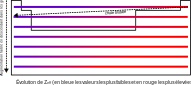
\includegraphics[scale=0.4]{evo_zeff}\includegraphics[scale=0.4]{evo_rcov}

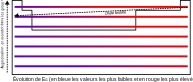
\includegraphics[scale=0.4]{evo_ei1}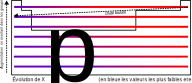
\includegraphics[scale=0.4]{evo_xp}

\section{Méthode}
%\subsection{Représenter la CEF sur un schéma avec les règles de Hund}
\subsection{Écire la CEF des Ions}
On écrit d'abord le neutre, puis on enlève l'électron après avoir classé les couche par $n$ croissant
\subsection{Déterminer le groupe et la période à partir de la CEF}
Dans le cas d'un ion on on donne la période et le groupe de l'atome.

La période correspond au $n$ le plus haut.

Le groupe correspond à la somme du nombre d'électrons de Valence. Si la période est $\leq 3$ et que le groupe trouvé est $\geq 3$, alors on ajoute 10 au groupe.
Faire méthode + pièges (+10, etc)
\subsection{Calculer l'énergie de première ionisation d'un élément}
On calcule l'énergie de l'atome puis celle de l'ion, et on les soustrait.
Pour cela, on somme l'énergie de chaque électrons.

Pour les électrons de la sous-couche $1s$, on calcule leur énergie : $-\frac{Z_{eff}(1s)^2\times 13.6}{1^2}$.

On calcule l'écrantage en se rappelant que l'électron ne s'écrante pas lui m\^eme.

On multiplie par le nombre d'électrons de la sous-couche.

On réitère pour les couches 2s/2p, 3s/3p, 3d, 4s/4d

Exemple : Cacluler l'énergie de ionisation du Beryllium

$Be : 1s^22s^2$

$E(Be) = -2\frac{Z_{eff}(1s)^2\times 13.6}{1^2} - 2$\marginTips{Le coefficient correspond au nombres d'électrons dans la/les sous-couches étudiée(s).}$\frac{Z_{eff}(2s/2p)^2\times 13.6}{2^2}$

On calcules les $Z_{eff}$ :

$Z_{eff}(1s) = 4-1\times 0.31 = 3.69$

$Z_{eff}(2s/2p) = 4-(2\times 0.85 + 1\times 0.35$\marginCritical{Il ne faut pas oublier d'ajouter l'écrantage des électrons de la m\^eme couche. Cet écrantage est multiplié par le nombre d'électrons dans la couche - 1 car un électron ne s'écrante pas lui m\^eme.}$) = 1.95$

Donc $E(Be) = -2\frac{(3.69)^2\times 13.6}{1^2} - 2\frac{(1.95)^2\times 13.6}{2^2} = -396 eV$

On calcule ensuite $E(Be^+) = -2\frac{Z_{eff}(1s)^2\times 13.6}{1^2} - 1\frac{Z_{eff}(2s/2p)^2\times 13.6}{2^2}$

L'écrantage des électrons de coeur reste identique, on calcule celui de la couche 2s/2p : $Z_{eff}(2s/2p) = 4-(2\times 0.85 + 0\times 0.35$\marginCritical{Il n'y a plus qu'un seul électron en 2s, donc on ne compte que l'écrantage des électrons en couche 1s}$) = 2.3$

Donc $E(Be^+) = -2\frac{(3.69)^2\times 13.6}{1^2} - 2\frac{(2.3)^2\times 13.6}{2^2} = -388 eV$

Donc $E_i = E(Be^+)-E(Be) = -388+396 = 8$ eV.
\subsection{Déterminer l'affinité électronique}

On calcule l'énergie de l'atome, comme indiqué dans la méthode précédente et celle de l'anion. L'affinité électronique est : $-(E(A)-E(A^-))$
\end{document}

